
\documentclass[letterpaper,hide notes,xcolor={table,svgnames},pdftex]{beamer}
\def\showexamples{t}


%\usepackage[svgnames]{xcolor}

%% Demo talk
%\documentclass[letterpaper,notes=show]{beamer}

\usecolortheme{crane}%seahorse crane
\setbeamertemplate{navigation symbols}{}

\usetheme{MyPittsburgh}
%\usetheme{Frankfurt}

%\usepackage{tipa}

\usepackage{hyperref}
\usepackage{graphicx,xspace}
\usepackage[normalem]{ulem}

\newcommand\SF[1]{$\bigstar$\footnote{SF: #1}}

\usepackage{paratype}
\renewcommand*\familydefault{\sfdefault} %% Only if the base font of the document is to be sans serif
\usepackage[zerostyle=c]{newtxtt}
\usepackage[T1]{fontenc}

\newcounter{tmpnumSlide}
\newcounter{tmpnumNote}

\usepackage{xcolor}
\usepackage{tabu}
\definecolor{light-gray}{gray}{0.75}
\taburulecolor{light-gray}

% old question code
%\newcommand\question[1]{{$\bigstar$ \small \onlySlide{2}{#1}}}
% \newcommand\nquestion[1]{\ifdefined \presentationonly \textcircled{?} \fi \note{\par{\Large \textbf{?}} #1}}
% \newcommand\nanswer[1]{\note{\par{\Large \textbf{A}} #1}}


 \newcommand\mnote[1]{%
   \addtocounter{tmpnumSlide}{1}
   \ifdefined\showcues {~\tiny\fbox{\arabic{tmpnumSlide}}}\fi
   \note{\setlength{\parskip}{1ex}\addtocounter{tmpnumNote}{1}\textbf{\Large \arabic{tmpnumNote}:} {#1\par}}}

\newcommand\mmnote[1]{\note{\setlength{\parskip}{1ex}#1\par}}

%\newcommand\mnote[2][]{\ifdefined\handoutwithnotes {~\tiny\fbox{#1}}\fi
% \note{\setlength{\parskip}{1ex}\textbf{\Large #1:} #2\par}}

%\newcommand\mnote[2][]{{\tiny\fbox{#1}} \note{\setlength{\parskip}{1ex}\textbf{\Large #1:} #2\par}}

\newcommand\mquestion[2]{{~\color{red}\fbox{?}}\note{\setlength{\parskip}{1ex}\par{\Large \textbf{?}} #1} \note{\setlength{\parskip}{1ex}\par{\Large \textbf{A}} #2\par}\ifdefined \presentationonly \pause \fi}

\newcommand\blackboard[1]{%
\ifdefined   \showblackboard
  {#1}
  \else {\begin{center} \fbox{\colorbox{blue!30}{%
         \begin{minipage}{.95\linewidth}%
           \hspace{\stretch{1}} Some space intentionally left blank; done at the blackboard.%
         \end{minipage}}}\end{center}}%
         \fi%
}



%\newcommand\q{\tikz \node[thick,color=black,shape=circle]{?};}
%\newcommand\q{\ifdefined \presentationonly \textcircled{?} \fi}

\usepackage{listings}
\lstset{%
  keywordstyle=\bfseries,
  aboveskip=15pt,
  belowskip=15pt,
  captionpos=b,
  identifierstyle=\ttfamily,
  escapeinside={(*@}{@*)},
  stringstyle=\ttfamiliy,
  frame=lines,
  numbers=left, basicstyle=\scriptsize, numberstyle=\tiny, stepnumber=0, numbersep=2pt}

\usepackage{siunitx}
\newcommand\sius[1]{\num[group-separator = {,}]{#1}\si{\micro\second}}
\newcommand\sims[1]{\num[group-separator = {,}]{#1}\si{\milli\second}}
\newcommand\sins[1]{\num[group-separator = {,}]{#1}\si{\nano\second}}
\sisetup{group-separator = {,}, group-digits = true}

%% -------------------- tikz --------------------
\usepackage{tikz}
\usetikzlibrary{positioning}
\usetikzlibrary{arrows,backgrounds,automata,decorations.shapes,decorations.pathmorphing,decorations.markings,decorations.text}

\tikzstyle{place}=[circle,draw=blue!50,fill=blue!20,thick, inner sep=0pt,minimum size=6mm]
\tikzstyle{transition}=[rectangle,draw=black!50,fill=black!20,thick, inner sep=0pt,minimum size=4mm]

\tikzstyle{block}=[rectangle,draw=black, thick, inner sep=5pt]
\tikzstyle{bullet}=[circle,draw=black, fill=black, thin, inner sep=2pt]

\tikzstyle{pre}=[<-,shorten <=1pt,>=stealth',semithick]
\tikzstyle{post}=[->,shorten >=1pt,>=stealth',semithick]
\tikzstyle{bi}=[<->,shorten >=1pt,shorten <=1pt, >=stealth',semithick]

\tikzstyle{mut}=[-,>=stealth',semithick]

\tikzstyle{treereset}=[dashed,->, shorten >=1pt,>=stealth',thin]

\usepackage{ifmtarg}
\usepackage{xifthen}
\makeatletter
% new counter to now which frame it is within the sequence
\newcounter{multiframecounter}
% initialize buffer for previously used frame title
\gdef\lastframetitle{\textit{undefined}}
% new environment for a multi-frame
\newenvironment{multiframe}[1][]{%
\ifthenelse{\isempty{#1}}{%
% if no frame title was set via optional parameter,
% only increase sequence counter by 1
\addtocounter{multiframecounter}{1}%
}{%
% new frame title has been provided, thus
% reset sequence counter to 1 and buffer frame title for later use
\setcounter{multiframecounter}{1}%
\gdef\lastframetitle{#1}%
}%
% start conventional frame environment and
% automatically set frame title followed by sequence counter
\begin{frame}%
\frametitle{\lastframetitle~{\normalfont(\arabic{multiframecounter})}}%
}{%
\end{frame}%
}
\makeatother

\makeatletter
\newdimen\tu@tmpa%
\newdimen\ydiffl%
\newdimen\xdiffl%
\newcommand\ydiff[2]{%
    \coordinate (tmpnamea) at (#1);%
    \coordinate (tmpnameb) at (#2);%
    \pgfextracty{\tu@tmpa}{\pgfpointanchor{tmpnamea}{center}}%
    \pgfextracty{\ydiffl}{\pgfpointanchor{tmpnameb}{center}}%
    \advance\ydiffl by -\tu@tmpa%
}
\newcommand\xdiff[2]{%
    \coordinate (tmpnamea) at (#1);%
    \coordinate (tmpnameb) at (#2);%
    \pgfextractx{\tu@tmpa}{\pgfpointanchor{tmpnamea}{center}}%
    \pgfextractx{\xdiffl}{\pgfpointanchor{tmpnameb}{center}}%
    \advance\xdiffl by -\tu@tmpa%
}
\makeatother
\newcommand{\copyrightbox}[3][r]{%
\begin{tikzpicture}%
\node[inner sep=0pt,minimum size=2em](ciimage){#2};
\usefont{OT1}{phv}{n}{n}\fontsize{4}{4}\selectfont
\ydiff{ciimage.south}{ciimage.north}
\xdiff{ciimage.west}{ciimage.east}
\ifthenelse{\equal{#1}{r}}{%
\node[inner sep=0pt,right=1ex of ciimage.south east,anchor=north west,rotate=90]%
{\raggedleft\color{black!50}\parbox{\the\ydiffl}{\raggedright{}#3}};%
}{%
\ifthenelse{\equal{#1}{l}}{%
\node[inner sep=0pt,right=1ex of ciimage.south west,anchor=south west,rotate=90]%
{\raggedleft\color{black!50}\parbox{\the\ydiffl}{\raggedright{}#3}};%
}{%
\node[inner sep=0pt,below=1ex of ciimage.south west,anchor=north west]%
{\raggedleft\color{black!50}\parbox{\the\xdiffl}{\raggedright{}#3}};%
}
}
\end{tikzpicture}
}


%% --------------------

%\usepackage[excludeor]{everyhook}
%\PushPreHook{par}{\setbox0=\lastbox\llap{MUH}}\box0}

%\vspace*{\stretch{1}

%\setbox0=\lastbox \llap{\textbullet\enskip}\box0}

\setlength{\parskip}{\fill}

\newcommand\noskips{\setlength{\parskip}{1ex}}
\newcommand\doskips{\setlength{\parskip}{\fill}}

\newcommand\xx{\par\vspace*{\stretch{1}}\par}
\newcommand\xxs{\par\vspace*{2ex}\par}
\newcommand\tuple[1]{\langle #1 \rangle}
\newcommand\code[1]{{\sf \footnotesize #1}}
\newcommand\ex[1]{\uline{Example:} \ifdefined \presentationonly \pause \fi
  \ifdefined\showexamples#1\xspace\else{\uline{\hspace*{2cm}}}\fi}

\newcommand\ceil[1]{\lceil #1 \rceil}


\AtBeginSection[]
{
   \begin{frame}
       \frametitle{Outline}
       \tableofcontents[currentsection]
   \end{frame}
}



\pgfdeclarelayer{edgelayer}
\pgfdeclarelayer{nodelayer}
\pgfsetlayers{edgelayer,nodelayer,main}

\tikzstyle{none}=[inner sep=0pt]
\tikzstyle{rn}=[circle,fill=Red,draw=Black,line width=0.8 pt]
\tikzstyle{gn}=[circle,fill=Lime,draw=Black,line width=0.8 pt]
\tikzstyle{yn}=[circle,fill=Yellow,draw=Black,line width=0.8 pt]
\tikzstyle{empty}=[circle,fill=White,draw=Black]
\tikzstyle{bw} = [rectangle, draw, fill=blue!20, 
    text width=4em, text centered, rounded corners, minimum height=2em]
    
    \newcommand{\CcNote}[1]{% longname
	This work is licensed under the \textit{Creative Commons #1 3.0 License}.%
}
\newcommand{\CcImageBy}[1]{%
	\includegraphics[scale=#1]{creative_commons/cc_by_30.pdf}%
}
\newcommand{\CcImageSa}[1]{%
	\includegraphics[scale=#1]{creative_commons/cc_sa_30.pdf}%
}
\newcommand{\CcImageNc}[1]{%
	\includegraphics[scale=#1]{creative_commons/cc_nc_30.pdf}%
}
\newcommand{\CcGroupBySa}[2]{% zoom, gap
	\CcImageBy{#1}\hspace*{#2}\CcImageNc{#1}\hspace*{#2}\CcImageSa{#1}%
}
\newcommand{\CcLongnameByNcSa}{Attribution-NonCommercial-ShareAlike}


\newenvironment{changemargin}[1]{% 
  \begin{list}{}{% 
    \setlength{\topsep}{0pt}% 
    \setlength{\leftmargin}{#1}% 
    \setlength{\rightmargin}{1em}
    \setlength{\listparindent}{\parindent}% 
    \setlength{\itemindent}{\parindent}% 
    \setlength{\parsep}{\parskip}% 
  }% 
  \item[]}{\end{list}} 




\title{Lecture 3 --- Hello World \& Simple Types }

\author{J. Zarnett\\
\texttt{jzarnett@uwaterloo.ca}}
\institute{Department of Electrical and Computer Engineering \\
  University of Waterloo}
\date{\today}

\begin{document}

\begin{frame}
  \titlepage
  
  \begin{center}
  \small{Acknowledgments: W.D. Bishop}
  \end{center}
 \end{frame}
 

\part{Hello World}
\begin{frame}\partpage\end{frame}

\begin{frame}
\frametitle{Hello World}

By longstanding tradition, the first program example when learning a new programming language is known as the \alert{Hello World} program.

All it does is write the text ``Hello World'' to the display device.

It is a simple program; easily understood.

It takes very little time to write and is hard to get wrong.

Successful execution of it proves that the environment, compiler, display system, etc. are all present and working.

\end{frame}

\begin{frame}[fragile]
\frametitle{Our First C++ Program}

\begin{verbatim}
#include <iostream>

using namespace std;

int main()
{
    cout << "Hello World!" << endl;
    return 0;
}
\end{verbatim}

\end{frame}

\begin{frame}
\frametitle{Examining the Hello World Program}
Let's examine each of the lines of this program.

At this point it is not expected that you will understand all the lines.

We'll say what they are, so more advanced students can understand the structure. If it's confusing to you, you will understand later.

What we are really interested in takes place between the inner set of \{ \} braces.

\end{frame}

\begin{frame}
\frametitle{Examining the Hello World Program}

\texttt{\#include <iostream>}\\
\quad This includes a header file for input/output purposes. Including the header file makes certain functions available for use in the program.

\texttt{using namespace std;}\\
\quad This indicates the use of functions in the std namespace.

\texttt{int main()}\\
\quad This is the entry point for program execution.

\texttt{cout << "Hello World!" << endl;}\\
\quad Tells the computer to output ``Hello World'' to the console.\\
\quad It also tells the computer to end the line and move to the next one.

\texttt{return 0;}\\
\quad Indicates this function is finished and its return value is zero.

\end{frame}

\begin{frame}
\frametitle{About Braces}

In the Hello World program, we see the \{ and \} braces.

These define a \alert{block}: a grouping of statements.

The \{ indicates the start of a block; \\
The \} indicates the end of that block.

They must be balanced (otherwise it's a syntax error).

\end{frame}

\begin{frame}
\frametitle{About Semicolons}

Examine: \texttt{cout << "Hello World!" << endl;}

Note the presence of a semicolon (\textbf{;}) at the end of that statement.

Often, a single statement appears on a line.

In C++, the semicolon denotes the end of many (but not all) statements.

The end of the line doesn't indicate the end of a statement.\\
This allows:\\
\quad\quad A statement to be on more than one line; or\\
\quad\quad More than one statement on a single line.

Forgetting a semicolon is a common syntax error.

\end{frame}

\begin{frame}
\frametitle{The \texttt{Main} Entry Point}

All languages provide an entry point for program execution.

The \alert{program entry point}  tells the compiler where to find the first instruction of a program.

There can be only one program entry point at compilation time.

\end{frame}

\begin{frame}
\frametitle{The \texttt{Main} Entry Point}


In C++, the simplest program entry point is defined as:\\
\quad	\texttt{int main( ) \{ \}}

Our code goes in the block between the \{ and \} braces after \texttt{main()}.

We can, for the moment, when creating a program, ignore all the other bits and just write our code inside this ``main'' block.

Later on, we'll understand all the parts.

\end{frame}

\begin{frame}
\frametitle{Writing \& Compiling the Program}
Programs are formed from source code: text written in a text file.\\
\quad The text is written in a language the compiler understands (C++).

By convention,  files containing C++ code use the file extension \texttt{.cpp}, such as \texttt{helloworld.cpp}

In this course, we will use the command-line compiler \texttt{gcc}.

To compile the program at the command prompt, use the command:\\
\quad \texttt{gcc filename.cpp}

\end{frame}

\begin{frame}
\frametitle{Compiling the Program}

If we compile the Hello World program, what is our output?

On the assumption that there were no syntax errors, the compiler will run and there will be no error output.\\
\quad You are left with a compiled, executable program.

If we made a mistake in writing the program, the compiler may identify it and report that to us.

[Demo: using the compiler; seeing successful/unsuccessful compiles]

\end{frame}

\begin{frame}
\frametitle{Compile-Time Errors}

If compilation did not succeed, we cannot run the program.\\
\quad Because no program was produced.

The compiler provides us with some error message(s) to identify why the compile was unsuccessful.

Read these messages carefully to find the error in the program.

Compiling again without fixing the error results in the same outcome.

After we correct the error, compile the program again.

\end{frame}

\begin{frame}
\frametitle{Running the Program} 
If compilation succeeded, an executable file was generated and we can run this file.

On the command line, we start execution by using the name of the executable.


By default, \texttt{gcc} names the output executable \texttt{a.out}.

\end{frame}

\begin{frame}
\frametitle{Program Execution}

When this program executes, it performs the following steps:

\begin{enumerate}
	\item Starts executing instructions at the start of \texttt{main( )}
	\item Executes \texttt{cout << "Hello World!" << endl;} displaying the ``Hello World'' text on the display
	\item Finishes execution: returns control to the operating system
\end{enumerate}

[Demo: running the program]

\end{frame}

\begin{frame}
\frametitle{Behind the Scenes of Hello World}

The implementation is straightforward in a high-level language.

It's easy for us to write, but for the computer it is complex.

It requires the execution of many machine language instructions.

Each character must be written to the screen at the right time.

Output statements equal many machine language instructions.

\end{frame}


\part{Simple Types}
\begin{frame}\partpage\end{frame}

\begin{frame}
\frametitle{Variables}
Flash back to high school algebra: variables.

Algebraic variables look like this: $x$

We often \alert{declare} a variable like so: Let $x = 5$.

Conceptually: $x$ is a quantity and at the moment, the value of $x$ is 5.

To conceptualize it visually, we have a box labelled $x$. \\ \quad The number in that box is 5.

\end{frame}

\begin{frame}
\frametitle{Variables}

Variables are changeable: later, we might say: Let $x = 7$.\\
\quad The number in the box changes to 7.

In algebra, you commonly saw expressions involving variables:\\
\quad $y = x + 1$

We have a new box, labelled $y$, and we evaluate $x + 1$.\\
\quad Because $x = 7$ and $7 + 1 = 8$, $y = 8$.\\
\quad Write $8$ into the box labelled $y$.

\end{frame}

\begin{frame}
\frametitle{Variables: Declaration}

We have the same idea in programming: software variables.

Conceptually it's the same idea: we \alert{declare} a variable.

When a variable is declared, the computer marks a memory location to represent that variable. 

That memory location is accessible by the name of the variable.

This is like creating a box and labelling it $x$ after we write ``Let $x$ = 5''

\end{frame}

\begin{frame}
\frametitle{Variables: Assignment}

When putting a value in the variable's box, we call that \alert{assignment}.

Assignment can set or change the value of the variable.

Sometimes we can declare a variable to be \alert{read-only}: we can set its value when we create it, but cannot change it after that.

\end{frame}

\begin{frame}
\frametitle{Variables: Type}

In algebra, a variable $x$ always contains a number (of some kind).

In some programming languages, when declaring a variable, it is necessary to specify a \alert{Type}.

The type tells the compiler and computer what kind of value is stored in the box.

Example: declaring a variable as an \alert{integer} (whole number).

\end{frame}

\begin{frame}
\frametitle{Variables: Type}

Why does the type matter? Some possible answers:

Tell the compiler how much space it takes to store the value.\\
\quad A big number, or one with high precision, takes more space to store.

Optimization: the compiler can translate your code into specialized instructions that operate on that data type rather than general ones.

Compile time checking: avoid assigning a ``wrong'' value to a variable.\\ \quad e.g., prevent assigning $1.5$ to a variable that should be an integer.

(Some languages don't care \& just figure things out at runtime. \\They do not benefit from this compile time checking.)

\end{frame}

\begin{frame}
\frametitle{Declaring a Variable}
The equivalent to our algebraic statement ``let $x = 5$'' in C++ code:\\
\quad \texttt{int x = 5;}

This statement follows the pattern \textit{type} \textit{identifier} = \textit{value;}

\texttt{int} is the type; it's a language keyword indicating an integer variable.

\texttt{x} is the identifier; it's the name of the variable (and is case-sensitive).

\texttt{5} is a literal; it's the explicit value being stored in the variable \texttt{x}.

\end{frame}

\begin{frame}
\frametitle{Initializing a Variable}
It's not strictly necessary to assign a value to \texttt{x} when it is declared.

\texttt{int x;}\\
\quad is acceptable as a declaration.

At some later time, we can set the value of this variable with an assignment statement:\\
\quad \texttt{x = 3;}

The first time a variable is assigned a value, we call that \alert{initialization}.

It is often an error to use an uninitialized (not set) variable.

\end{frame}

\begin{frame}
\frametitle{Read-Only Variables}
To declare a variable as read-only, we use the keyword \alert{\texttt{const}}.\\
\quad Example: \texttt{const int c = 0;}

If we mark a variable as \texttt{const}, it means that after assigning a value to that variable, we may not change it later.\\
\quad A later attempt to assign \texttt{ c = 1; } is a compile-time error.

\end{frame}

\begin{frame}
\frametitle{C++ Built-In Data Types}

C++ has many different variable types.

Most of them refer to different types of numbers.

There are other values we can store in variables, but we'll examine numbers first.


\end{frame}

\begin{frame}
\frametitle{C++ Built-In Numeric Types}
\begin{center}
{\scriptsize
\begin{tabular}{l|l}
\textbf{Type} & \textbf{Description}\\ \hline
\texttt{short int} & Signed 16-bit integer\\ \hline
\texttt{unsigned short int} & Unsigned 16-bit integer\\ \hline
\texttt{int} & Signed 16-bit integer\\ \hline
\texttt{unsigned int} & Unsigned 16-bit integer\\ \hline
\texttt{long int} & Signed 32-bit integer\\ \hline
\texttt{unsigned long int} & Unsigned 32-bit integer\\ \hline
\texttt{long long int} & Signed 64-bit integer\\ \hline
\texttt{unsigned long long int} & Unsigned 64-bit integer\\ \hline
\texttt{float} & Signed 32-bit floating point\\ \hline
\texttt{double} & Signed 64-bit floating point\\ \hline
\texttt{long double} & Signed 80-bit extended precision floating point\\
\end{tabular}
}
\end{center}

Note that the number of bits are the minimum bits; it varies by platform.

In particular, in most cases, the regular \texttt{int} is 32 bits.

\end{frame}

\begin{frame}
\frametitle{C++ Built-In Numeric Types}

\begin{center}
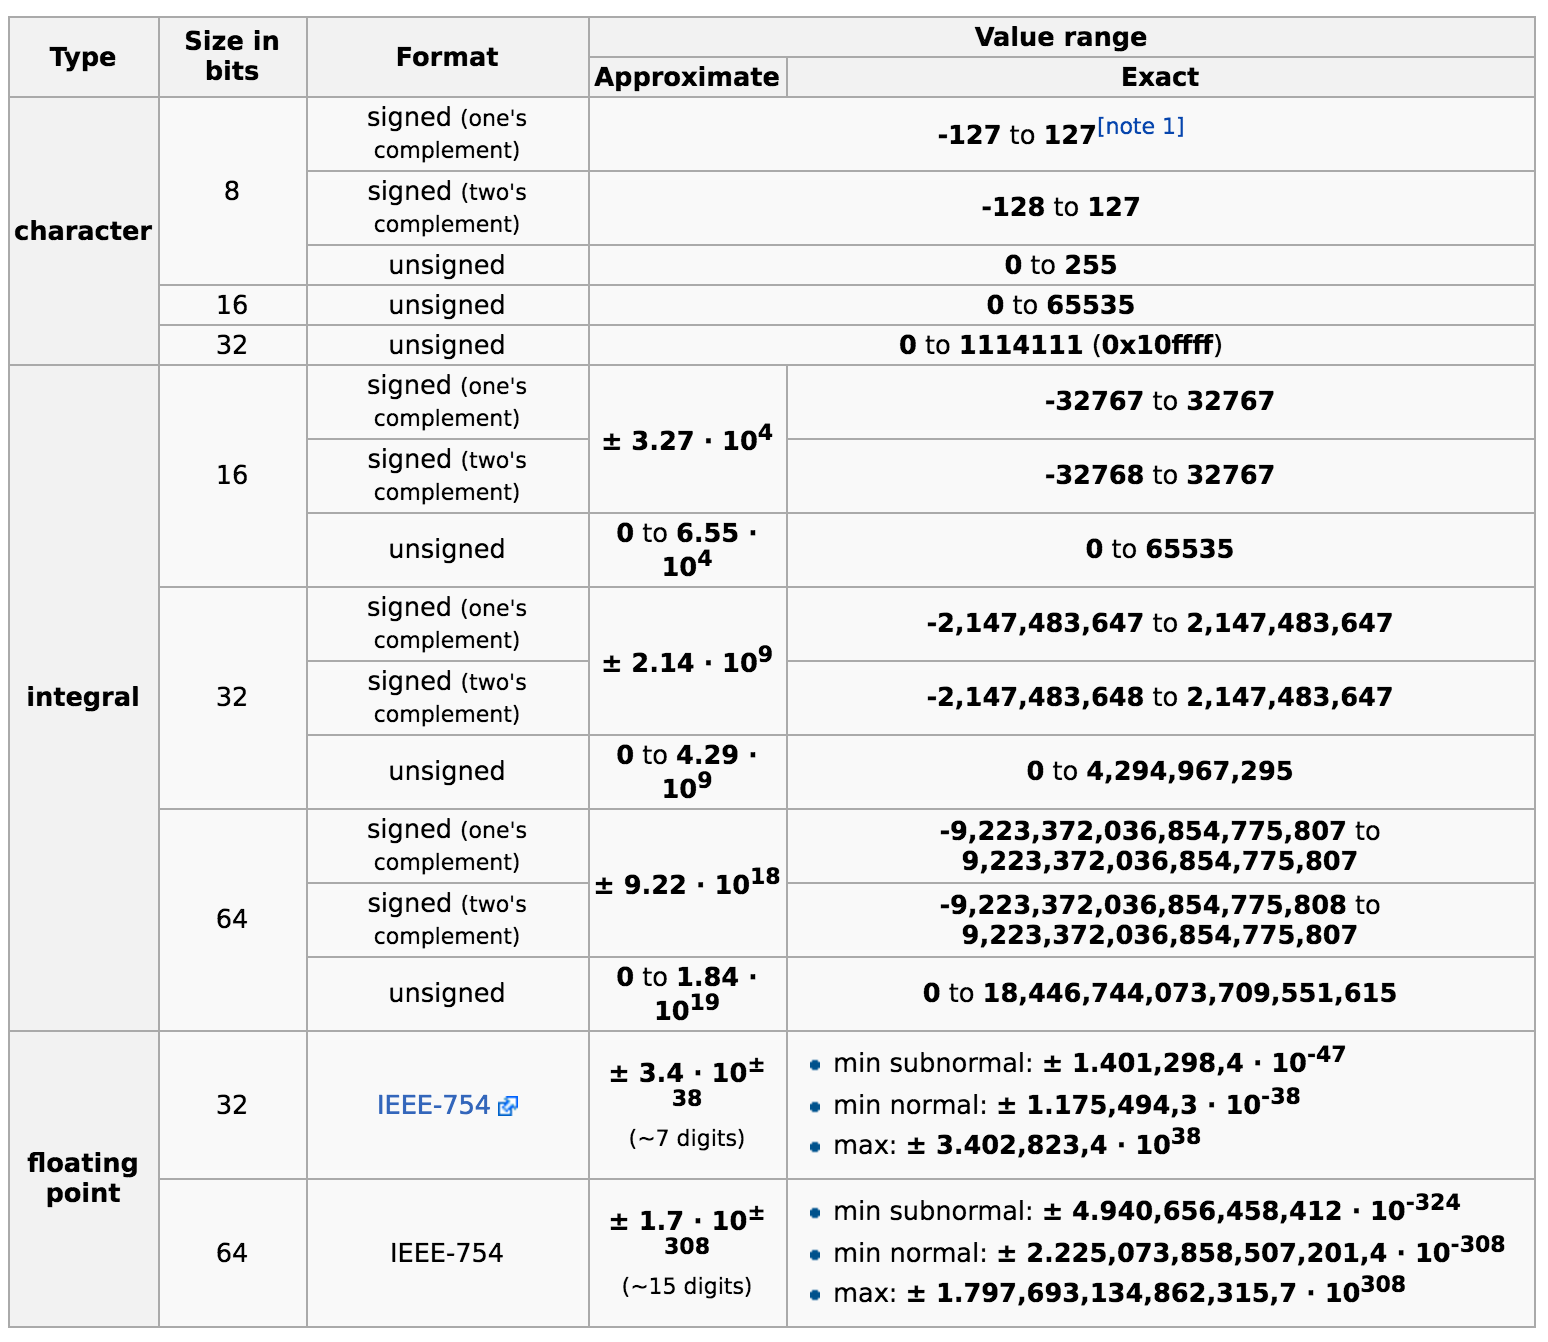
\includegraphics[width=.78\textwidth]{images/cppvaluerange.png}\\
{\scriptsize Source: \url{http://en.cppreference.com/w/cpp/language/types}}
\end{center}



\end{frame}

%\begin{frame}
%\frametitle{C\# Built-In Numeric Types}
%{\scriptsize
%\begin{center}
%\begin{tabular}{l|l|r|r}
%\textbf{Type} & \textbf{Epsilon Value} & \textbf{Minimum Value} & \textbf{Maximum Value} \\
% & (Min. Change) & & \\ \hline
%\texttt{byte} & $\pm$ 1 & 0 & +255 \\ \hline
%\texttt{ushort} & $\pm$ 1 & 0 & +65,535 \\ \hline
%\texttt{uint} & $\pm$ 1 & 0 & +4,294,967,295 \\ \hline
%\texttt{ulong} & $\pm$ 1 & 0 & +18,446,744,073,709,551,615 \\ \hline
%\texttt{sbyte} & $\pm$ 1 & -128 & +127 \\ \hline
%\texttt{short}  & $\pm$ 1 & -32,768 & +32,767 \\ \hline
%\texttt{int} & $\pm$ 1 & -2,147,483,648 & +2,147,483,647 \\ \hline
%\texttt{long} & $\pm$ 1 & -9,223,372,036,854,775,808 & +9,223,372,036,854,775,807 \\ \hline
%\texttt{float} & $\pm$ 1.5 x $10^{-45}$ & -3.4 x $10^{+38}$ & +3.4 x $10^{+38}$ \\ \hline
%\texttt{double} & $\pm$ 5.0 x $10^{-324}$ & -1.7 x $10^{+308}$ & +1.7 x $10^{+308}$ \\ \hline
%\texttt{decimal} & $\pm$ 1.0 x $10^{-28}$ & -7.9 x $10^{+28}$ & +7.9 x $10^{+28}$ \\
%\end{tabular}
%\end{center}
%}
%\end{frame}

\begin{frame}
\frametitle{Assigning Numeric Types}

When assigning the numeric types in code, we often use literals like 5.

Literals may need a letter (or two) after them to tell the compiler the format of the literal.

If you don't specify, the compiler will try to guess what you meant.

\end{frame}

\begin{frame}
\frametitle{C++ Number Formats}

\begin{itemize}
	\item Unsigned numbers are followed by U or u\\ \quad
Examples: 5U, 5u, etc.
	\item Long numbers are followed by L or l\\ \quad
Examples: 5L, 5l, 362.f12L etc.
	\item Single-precision, floating point numbers are followed by F or f\\ \quad
Examples: 362.5F, 362.5f, etc.
\end{itemize}

\end{frame}

\begin{frame}
\frametitle{C++ Number Formats}

We can also express numbers with powers of 10.

The double-precision floating point value for 3.625 x $10^{2}$ can be expressed as \texttt{3.625E2D} or \texttt{3.625e2d}.


Assignment statements would therefore look like:

\texttt{long example1 = 900l;}

\texttt{float example2 = 365.25f;}

\texttt{double example3 = 75.5e4;}


\end{frame}


\begin{frame}
\frametitle{Too Many Number Types!}

There are a lot of choices, but it turns out in practice you are likely to use just a small number of them.

Typically \texttt{int} and \texttt{double} are the most common choices for integer and real (floating point) numbers.

Other types have their applications, however.

\end{frame}

\begin{frame}
\frametitle{Other Simple Types}

Aside from numbers, there are 2 other simple types to examine today.

The \texttt{bool} (boolean variable); and \\
The \texttt{char} (character).

\end{frame}

\begin{frame}
\frametitle{Boolean Variables}

A \texttt{bool} defines a Boolean variable.

A Boolean variable can only have one of two possible values: \\
\quad \texttt{true} or \texttt{false}.

In C++, Boolean variables may be assigned values of 0 or 1.\\
\quad But this is not recommended.

Example: \texttt{bool printingEnabled = true;}

\end{frame}

\begin{frame}
\frametitle{C++ Character Variables}

A \texttt{char} defines a character variable.

A character is a single symbol from an alphabet, like 'a', 'z', or a Japanese kanji.

A \texttt{char} literal is enclosed in single quotation characters (\texttt{'}).

Some examples of valid \texttt{char} declarations:

\texttt{char myChar1 = 'X';}  -- Character Literal\\
\texttt{char myChar2 = '\textbackslash x0058';} -- Hexadecimal\\
\texttt{char myChar3 = '\textbackslash u0058';} -- Unicode

A character can also be used to represent a numeric quantity.

\end{frame}

\begin{frame}[fragile]
\frametitle{Use of C++ Character Variables}

\begin{verbatim}
#include <iostream>

using namespace std;

int main()
{
    char myChar1 = 'X';
    char myChar2 = '\x0058';
    char myChar3 = '\u0058';

    cout << myChar1 << myChar2 << myChar3 << endl;
    return 0;
}
\end{verbatim}


[In-Class Demo: the output of this program]

\end{frame}

\begin{frame}
\frametitle{Console Output}

This is the second time (after the Hello World) program that we've seen console output (\texttt{cout} statements).

In the next lecture, we'll look at how console input and output work.

\end{frame}

\end{document}

